\cotefile{23}
\scanpage{51}

% letterhead
\begin{center}
INSTITUT\\
DES HAUTES ÉTUDES SCIENTIFIQUES\\
\rule{1.4cm}{0.4pt}
\end{center}

\uline{\unsure{Applications|Application} de 11.2.9.} dans la suite du Chap.~$\overline{\underline{\mathrm{IV}}}$

\[
\begin{aligned}
&11.3.4.\ \unsure{b\mathrm{i}|b_{\mathrm{i}}|(\mathrm{i}})\\
&11.3.8.\ b')\\[3pt]
&17.12.1.\ c')\\
&19.2.4.\ c')\\
&19.4.6.\ c\mathrm{ii})
\end{aligned}
\]

\uline{À signaler \deleted{\unsure{aux|en}}} \uline{\unsure{remarques|remarquer}} ?
% archive sheet number: 50
\scanpage{52}

% letterhead
\begin{center}
INSTITUT\\
DES HAUTES ÉTUDES SCIENTIFIQUES\\
\rule{1.4cm}{0.4pt}
\end{center}

\uline{Suites régulières, \unsure{immers.|imm.|immersions} régulières}

\[
\begin{aligned}
&0_{\overline{\underline{\mathrm{IV}}}} &&15\\
&\overline{\underline{\mathrm{IV}}} &&11.\unsure{3|7}.7.\qquad 11.3.8.\\
&\overline{\underline{\mathrm{IV}}} &&16.9.\\
&\overline{\underline{\mathrm{IV}}} &&19.\\
&\overline{\underline{\mathrm{IV}}} &&21.15.
\end{aligned}
\]

Lettres Deligne 17. Oct. 66. et 29 Oct. \deleted{\unsure{0}}66.

\deleted{Notion d'immersion régulière dans le cas non \unsure{noethérien} : est-elle \unsure{raisonnable|vraisemblable} ?? Vérifier \S~16 !!}
% archive sheet number: 51
\scanpage{53}

PS\quad Dans mon séminaire sur Riemann-Roch cette année, on doit mani\deleted{f}puler
systématiquement les immersions régulières dans le cas non noethérien,
et il apparait (hélas) que la notion introduite so\uline{u}s ce nom dans EGA
16.9.2. n'est pas la bonne notion. Un premier canular important, c'est
que si $A$ est un anneau local, et $x,y$ deux éléments de son idéal maximal,
il est facile de donner un exemple ou $(x,y)$ est une suite régulière,
et $(y,x)$ ne l'est pas. La notion de suite régulière de générateurs d'un
idéal ne jouit donc pas du tout des propriétés habituelles, comme
celle qu'il suffise de prendre une base de $J/J^2$ et de relever . Par suite,
la notion d'immersion régulière n'a pas l'air de \unsure{devoir s e|devoirs e|devoir se} comporter
comme il faut par localisation plate ou même étale, ce qui est un autre
grave inconvénient, en entrainant toute sorte d'autres d'ailleurs. Il
apparait maintenant que la notion vraiment serviable pour une suite
$(f_1,..,f_n)$ d'éléments d'un anneau (engendrant un idéal $J$) c'est que
le complexe de l'algèbre extérieure construit avec soit nul en degrés
$0$. Alors on prouve que la suite est aussi quasi-régulière, et de
plus que toute autre suite de \inserted{$n$} générateurs de $J$ a la même propriété
que celle énoncée pour $(f_1,..,f_n)$. Il y aurait lieu alors de dire que
$J$ est un idéal régulier si localement il peut être engendré par une
suite comme dessus (qu'on pourrait peut-être app\deleted{\unsure{e}}ler ``suite Koszul-régulière'' ou ``essentiellement régulière'', si on tientà ne pas changer la
terminologie des \uline{suites} régulières), et à définir de façon correspondante
la notion d'immersion régulière. Ces notions (suite K-régulière,
idéal régulier, immersion régulière) se descendent bien par fpqc. Un
composé de deux immersions régulières est itou, et les deux autres
propriétés de transitivité de 19.1.5. (iii) revu semblent marcher
encore sans hypothèse noethérienne (Berthelot en a déjà vérifié une,
% archive sheet number: 52
\scanpage{54}

en tous cas. De plus, bien entendu, pour ce qu'on veut en faire pour
R.R. , c'est bien la nouvelle notion d'immersion régulière qu\deleted{\unsure{e}}i fait
tout marcher.

Du point de vue pratique, il me semble évidemment trop tard pour
faire les changements désirables sur épreuves dans IV 16,19. On peut
cependant ajouter une remarque 19.1.8.,dans laquelle nous ferions l'aveu
\margin{\handwritten{\rule{0.25pt}{4.8cm}\hspace{2pt}\rule{0.25pt}{4.8cm}}}que \deleted{\unsure{la|ln}} la définition adoptée dans le texte de immersion régulière \deleted{n}s'est
\deleted{pas} avérée peu maniable dans le cas non noethérien, et qu'il y aurait
lieu de la modifier comme je viens de le dire, en\deleted{\unsure{r|é}} référant le lecteur
intéressé, \inserted{pour des détails} en attendant la réédition du Chap IV des EGA, au séminaire
SGA 6 (qui devrait sortir vers la fin de l'année 67 ou début 68). De
plus, à l'endroit du par.16 ou on introduit la définition inc\deleted{\unsure{i}}riminée,
nous pourrions insérer une note de bas de page, renvoyant le le cteur
à la remarque 19.1.8. concernant cette définition. (NB Dans le par.16,
c'est en fait la notion quasi-régulière qui sert vraiment ...).

Au moment de la réédition du Chap IV, il y aura lieu également de
revoir $0_{\mathrm{IV}}$ 15 dans le même esprit; je prévois que l'on pourra également
y remplacer partout les hypothèses ``suite régulière'', par l\deleted{a}'hypothèse
plus faible et plus maniable ``suite Koszul-régulière''. S'il en est
bien ainsi, il s'imposera alors, pour les suites également, de réserver
le mot le plus court à la notion qui manifestement est la plus serviable,
et il faudra envisaher de changer \deleted{\unsure{not|mot}} notre terminologie, en disant
``suite régulière'' au lieu de ``suite Koszul-régulière'', et en réservant
tout au plus un terme tel que ``suite strictement régulièr\deleted{\unsure{e|s}}e'' à la notion
éculée. Bien sûr, dans le cas noethérien, les trois variantes (régulière,
quasi; et Koko) sont équivalentes.
% archive sheet number: 53
\scanpage{55}

\hfill Lettres Deligne
% archive sheet number: 54
\scanpage{56}

Bruxelles 5, le 15 décembre 1966\\

Cher Grothendieck,\\

Je lis aujourd'hui ta lettre du 28 - Après avoir tourné 7 fois ma langue dans ma bouche, je réjète mon objection à l'hypothèse ``tout quotient de tout sous-module de $M$ est separé pour la topologie $J$-adique'', qui \uline{n'est pas}\inserted{ en général} vérifiée pour $M$ de type fini sur \deleted{\unsure{B}}la $A$-algèbre $B$, $A$ et $B$ noethériens, $JB\subset R(B)$.

\[
\begin{aligned}
&\text{\uline{Contre exemple} :}\quad A\ \text{noethérien local},\quad J=m\\
&\hphantom{\text{Contre exemple :}\quad} B=A[[T]],\quad M=B
\end{aligned}
\]

comme \uline{$A$-module}, $B\sim A_s^N$, donc tout module quotient de $A_s^{(N)}$ est quotient d'un sous-$A$-module de $B$. \deleted{\unsure{$T$|7|Un}} Un module ayant un système dénombrable de générateurs n'a aucune raison d'être séparé !

Bien sûr, les démonstrations \deleted{ne} n'utilisent que des quotient et sous-modules comme $B$-modules.

J'essayerai encore une fois de lire 19.7.

Bien à toi\\

P. Deligne\\

P.S. Je rappelle que l'adresse où tu me touches le plus rapidement est :

S.M.\quad P. Deligne\\
Athénée Royal de Rösrath\\
BPS 8\\
FBA - (forces belges en Allemagne)\\

P.S. Je commence à lire $\overline{\underline{\mathrm{IV}}}$ \S\,16. La démonstration de 16.1.5 est canulée, comme on le voit en prenant $X=\operatorname{Spec}(k[T])$, $Y=\operatorname{Spec}(k[T])\amalg\operatorname{Spec}(k)$, tous deux affins.

\diagram{\begin{tikzcd}[ampersand replacement=\&,row sep=2pt,column sep=2pt]
Y\arrow[d,xshift=-9pt] \& \left\{\ 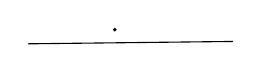
\begin{tikzpicture}[baseline=0pt]\draw (0,0)--(2.6,0.03);\fill (1.1,.18) circle (.025);\end{tikzpicture}\right.\\
X \& \left\{\ 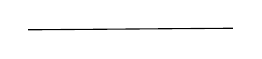
\begin{tikzpicture}[baseline=0pt]\draw (0,0)--(2.6,.02);\end{tikzpicture}\right.
\end{tikzcd}}

Avec les notations de 16.1.15 (\unsure{1|i}), $J=0$, mais les voisinages infinitésimaux de $Y$ ne sont pas \deleted{\unsure{nuls en $\operatorname{Spec}(k)$}} triviaux en $\operatorname{Spec}(k)$

J'ignore si la proposition est vraie -
% archive sheet number: 55
\scanpage{57}

Par ailleurs, même en admettant 16.1.5, 16.1.6 n'est pas convaincant en général : si $B$ est de présentation finie sur $A$, j'ignore si le noyau de $A\longrightarrow B$ est un idéal de type fini . C'est sans doute faux -
% archive sheet number: 56
\scanpage{58}

Rösrath, le 29 octobre 1966\\

\margin{\unsure{original}}

Cher Grothendieck,\\

Je te signale tout d'abord mon adresse en Allemagne, maintenant définitive (jusqu'au $1^{\underline{\mathrm{er}}}$ juillet 67)

S.M.\quad Pierre Deligne\\
Athénée royal\\
BPS 8\\
FBA (forces belges en Allemagne)\\

Je suis en train de lire EGA IV 19 que tu m'as envoyé.

\uline{a) remarque sur les hypothèses de séparation utilisées}

L'hypothèse $(*)$ ``tout quotient de tout sous-module de $M$ \deleted{\unsure{est}} (\deleted{resp} $M^n$) est séparé pour la topologie $J$-adique'' me semble idiote :

(i) elle \deleted{n'implique pas} n'est pas impliquée par l'hypothèse de finitude relative noethérienne standart : ``$M$ fini sur la $A$-algèbre noethérienne $B$, $A$ noethérien, et $JB\subset R(B)$'' qui elle est naturelle.

\margin{?\ \rule{0.25pt}{1.4cm}}

\margin{\uline{Err}}

(ii) le seul exemple non trivial indiqué où cette hypothèse est vérifiée, soit 19.5.6 (ii), est canulé, car \deleted{$(*)$} dans $(*)$ on ne se limite pas à prendre des quotients par des sous-modules gradués.

% slanted
\margin{\uline{\unsure{Ça va pas|ça va p.|ja \illegible{1}}}\ $\Big($}

\margin{?}

[exemple : $A=B[T]$, $M=N[T]$, $\deleted{\unsure{M}}N$ est un $A$-module, $T$ agissant par $1$, et ce $A$-module est quotient de $M$ ]

Je crois qu'il faut éviter d'employer des hypothèses de séparation qu'on ne rencontre pas dans la nature, comme ``idéalement séparé'' etc., et se limiter à utiliser (i) - J'avoue toutefois, avec honte, que dans le même geste sacrilège je serais prêt à supposer tous les schémas séparés et noethériens...

Sinon, pour coiffer (\unsure{i|1}) et $(*)$ resp. on pourrait prendre :

\margin{!\ $\Bigg($}

\[
\begin{aligned}
&\forall f:\ N\longrightarrow \deleted{\unsure{M}}P,\quad \text{si } N \text{ et } \deleted{\unsure{M}}P \text{ sont finis sur } A,\quad \operatorname{Ker}(M\otimes N\deleted{)}\longrightarrow\deleted{\operatorname{Ker}}\deleted{(}M\otimes P)\quad\text{est}\\
&\quad J\text{-séparé.}
\end{aligned}
\]
% archive sheet number: 57
\scanpage{59}

\uline{b) réponse à 19.5.6. (iii)}

L'implication $b)\Rightarrow c)$ de 19.5.5 est vraie sans qu'on doive faire aucune hypothèse de séparation. Pour le voir, il suffit de lire le cas $n=1$ de la démonstration ``à la Schwartz''.

Vu l'urgence que tu m'as signalée, et bien qu'il soit peut-être trop tard, je joins une rédaction de la démonstration (copiée sur la primitive)

--- Je n'ai pas encore compris 19.7.

--- J'ai beaucoup aimé le projet EGA I \S\,0 jusqu'à la pg 10, où la topologie du spectre tombe du ciel. Ne faudrait-il pas parler de topologie avant de parler d'espace topologique ?

--- Je ne suis pas capable de rédiger une théorie naïve utilisable d\deleted{\unsure{'}}es intersections, et n'ai pas d'autre remarque à faire sur le ``plan des EGA'' pour le moment

Bien à toi\\

P. Deligne\\
% archive sheet number: 58
\scanpage{60}

Bruxelles 5, le 17 octobre 1966\\

Cher Grothendieck,\\

J'ai bien reçu ta lettre.

Je n'ai pas l'intention d'essayer de démontrer, cette année, le ``théorème de \unsure{Lefschetz|Lefchetz} vache''. J'espère donc que tu trouves quelqu'un qui le fasse.

J'ai été malade au début du mois et, comme lecture de convalescence, je lis EGA $\overline{\underline{\mathrm{IV}}}$. Je ne sais pas si tu collectionnes déjà les \unsure{erratas|errata} et compléments pour EGA $0_{\overline{\underline{\mathrm{IV}}}}$ ; je t'envoie toujours ceux qui suivent.

$0_{\overline{\underline{\mathrm{IV}}}}$\quad 19.3.12

\margin{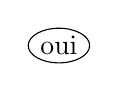
\begin{tikzpicture}[baseline=(n.base)]\node[inner sep=2pt](n){oui};\draw (n.center) ellipse (.39cm and .22cm);\end{tikzpicture}}

est \uuline{canulé} : il faut prendre pour $W_{\unsure{\lambda|s}}$ l'ensemble des homomorphismes d'\uline{algèbre} $B\longrightarrow C_\lambda$ qui relèvent $B\longrightarrow C_\lambda/J_\lambda$, et ce n'est pas une variété linéaire [on n'a pas $J_\lambda^2=0$] - Pour faire marcher l'argument, il faudrait savoir que pour $A$ artinien, l'ensemble des parties de $A^I$ définie par \deleted{\unsure{un syst.}} des équations $P(x_i)\in b$ ($b$ idéal) jouit d'une propriété de compacité. C'est faux pour $I$ infini, déjà pour $A$ un corps infini [$I=k\cup\{\infty\}$, parties $(x_\infty-u)y_u=1$, les $\cap$ finies sont non vides, l'$\cap$ est vide ] - Je crois qu'il n'y a pas d'espoir.

$0_{\overline{\underline{\mathrm{IV}}}}$\quad 17.3.4

Je te signale une jolie démonstration cohomologique de ce résultat, qui fournit un résultat plus complet (lequel se trouve dans Northcott)

\margin{(Th. de Auslander)}

\uline{prop} : $A$ \uline{local noethérien}, $M$ de type fini sur $A$, non nul, et de \uuline{dimension projective finie}. Alors $\underline{\dim\operatorname{proj}(M)=\operatorname{prof} A-\operatorname{prof} M}$.

On utilise la formule suivante, valable pour un complexe parfait $L$ .

\[
\operatorname{RHom}(K,L)=\operatorname{RHom}(K,A)\overset{L}{\otimes}L
\]

avec $K=k$, $L=M$. On trouve une suite spectrale

\[
E_2^{pq}=\operatorname{Tor}_{-p}(\deleted{\unsure{\operatorname{Tor}}}\operatorname{Ext}^{q}(k,A),M)\Longrightarrow \operatorname{Ext}^{p+q}(k,M).\qquad \text{(dessin ci contre)}
\]

\figure{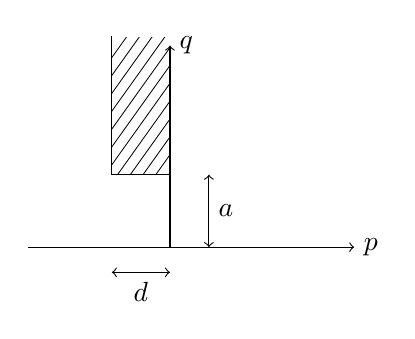
\begin{tikzpicture}[x=0.9cm,y=0.8cm]
\draw[->] (-2,0)--(2.6,0) node[right] {$p$};
\draw[->] (0,0)--(0,3.2) node[right] {$q$};
\draw (-.82,3.35)--(-.82,1.15)--(0,1.15);
\begin{scope}\clip (-.82,1.15) rectangle (0,3.32);
\foreach \a in {-2,-1.82,...,0.2} \draw[line width=.3pt] (\a,1.15)--++(1.65,2.6);
\end{scope}
\draw[<->] (-.82,-.4)--(0,-.4) node[midway,below] {$d$};
\draw[<->] (.55,0)--(.55,1.15) node[midway,right] {$a$};
\end{tikzpicture}}

si $d=\dim\operatorname{proj}M$, $a=\operatorname{prof}A$, on trouve

\[
\begin{aligned}
&\operatorname{Ext}^{n}(k,M)=0\quad\text{si }n<a-d\quad\text{et}\\
&\operatorname{Ext}^{a-d}(k,M)=\operatorname{Tor}_d(\operatorname{Ext}^a(k,A),M)\quad\text{, non nul}
\end{aligned}
\]

par hypothèse (car $\operatorname{Ext}^a(k,A)$ est somme de copies de $k$)

D'où la profondeur de $M$ ...
% archive sheet number: 59
\scanpage{61}

\mspage{2}

Le même résultat, \inserted{en remplacant $\dim\operatorname{proj}$ par $\operatorname{Tor}\dim$} est encore valable pour $M$ de type fini sur un anneau \deleted{\unsure{local $B$|local N|local}} noethérien $B$, qui soit une $A$-algèbre telle que $mB\subset\operatorname{radical}(B)$

Il faut savoir\quad (i) qu'on peut encore définir la profondeur de $M$ sur $A$ dans ce cas

(ii) que la Tor dimension de $M$ est le plus grand entier $d$ tel que $\operatorname{Tor}^d(k,M)\ne0$, où $k$ est le corps résiduel de $A$.

C'est là une conséquence facile du résultat suivant, pour lequel je ne connais pas de référence :

\uline{prop} : Soit $A$ un anneau \uline{local noethérien}, $\deleted{\unsure{A}}B$ une $A$-algèbre locale noethérienne ($A\longrightarrow B$ étant local), \uline{$m$ un idéal de $A$}, \uline{$\deleted{M}N$ un $A$-module de type fini}, \uline{$M$ un $\deleted{A}B$-module de type fini}. On a

\[
\underline{\varprojlim\operatorname{Tor}^{p}_{A}(N/_{m^kN},M)=
\operatorname{Tor}^{p}_{A}(N,M)^{\wedge}}\qquad\text{et plus précisément}
\]

une égalité de proobjets

\[
\text{``}\varprojlim\text{''}\ \operatorname{Tor}^{p}_{A}(N,M)\big/_{m^k\operatorname{Tor}^{p}(N,\unsure{M|N})}
\xrightarrow{\sim}\ \text{``}\varprojlim\text{''}\ \operatorname{Tor}^{p}_{A}(N/_{m^kN},M)
\]

Si $B$ était plat sur $A$, on prendrait une résolution de $\deleted{\unsure{N}}M$ sur $B$, et il suffirait d'appliquer Artin-Rees, qui exprime que ``le pro-objet complétion'' est foncteur exact. On peut par ailleurs remplacer $B$ par une algèbre dont il soit quotient. On peut aussi compléter $B$. L'assertion résulte alors du lemme suivant, qui coiffe

$0_{\overline{\underline{\mathrm{IV}}}}$ 19.7.1.3\\
et\\
$0_{\overline{\underline{\mathrm{III}}}}$ 10.3.1

\uline{prop} : Soit $A\longrightarrow B$ un homomorphisme local d'\uline{anneaux locaux noethériens}, avec \uuline{$B$ complet}. $B$ est quotient d'un $A$anneau $C$, tel que

% slanted
\margin{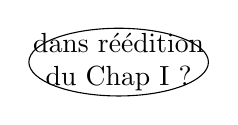
\begin{tikzpicture}[baseline]\node[align=center,inner sep=2pt] (m) {dans réédition\\du Chap I ?};\draw (m.center) ellipse (1.14cm and .43cm);\end{tikzpicture}}

(i) $C$ est local, $A\longrightarrow C$ et et $C\longrightarrow B$ sont locaux

(ii) \uline{$C$ est plat sur $A$}

(iii) Si $k$ est le corps résiduel de $A$, $C_0=C\otimes_A k$, $B_0=B\otimes_A k$, \uline{$C_0$ est un anneau \deleted{de séries formelles sur une extension $K$ de $k$}}\inserted{ régulier}, et l'application graduée associée à $C_0\longrightarrow B_0$ : $\operatorname{gr}C_0\longrightarrow\operatorname{gr}B_0$ est bijective en degré $0$ et $1$

\uline{Démonstration} : Soit $m$ ($n$) l'idéal maximal de $A$ ($B$), $K$ le corps résiduel de $B$.

Soit $t_i$ une base d'un supplémentaire de l'image de $m/_{m^2}\otimes_k K\longrightarrow n/_{n^2}$. Si on relève les $t_i$ dans $B$, on définit une flèche $A[[T_i]]\longrightarrow B$. Soit $A'=A[[T_i]]$, $m'$ son idéal maximal, $A'$ est plat sur $A$, et on a \deleted{\unsure{$m'/m'^2$}}

\[
m'/_{m'^2+mA'}\xrightarrow{\sim} n/_{n^2+mB}.
\]
% archive sheet number: 60
\scanpage{62}

\mspage{3}

Remplacant $A$ par $A'$, il reste à prouver que si $m/_{m^2}\otimes K\longrightarrow n/_{n^2}$ est surjectif \inserted{i é $K=B\otimes k$} on peut trouver $C$ tel que $K=C\otimes k$\inserted{ d'où $\operatorname{gr}C=K\otimes_k\operatorname{gr}A$}. On va manger $K$ par étapes

a) soit $(x_i)_{i\in I}$ une base de transcendance de $K$ sur $k$ ; \deleted{et} on relève les $x_i$ en des éléments de $B$, définissant ainsi $A(x_i)\longrightarrow B$. $A(x_i)$ est la limite inductive des localisées, au point générique de la fibre spéciale, des $A[X_i]_{i\in J}$, $J$ fini ds $I$. (cf Nagata, local rings pg 17 et 18). On peut soit utiliser $0_{\overline{\underline{\mathrm{III}}}}$ 10.3.1.3 pour vérifier que cet anneau est noethérien, soit le compléter et utiliser le critère de platitude pour vérifier que son \unsure{complété|complétée} est plat sur $A$

b) on s'est ainsi réduit à supposer $K$ algébrique sur $k$ et, si on y tient, à supposer $A$ complet. On trouve sans histoire $A'$ plat sur $A$, non ramifié, de corps résiduel la cloture séparable de $k$ dans $K$, et $A'\longrightarrow B$. Reste à traiter le cas où $K/k$ est purement inséparable, et on va utiliser une propriété ``d'intersection complète'' des corps, que je n'ai pas su bien dégager

c) on suppose : $K/k$ purement inséparable, $A$ et $B$ complets, $\deleted{\unsure{B}}K=\deleted{\unsure{A}}B\otimes k$.

soit $K_n$ le sous corps de $K$ formé des $x$ tels que $x^{p^n}\in k$ ($K_n=K\cap k^{p^{-n}}$), et soit $x_n^\alpha$ une $p$-base de $K_n$ sur $K_{n-1}$ ($n\geq1$). $K$ est \deleted{\unsure{le}} l'anneau engendré par des éléments $x_n^\alpha$ soumis à des relations $(x_n^\alpha)^p=P_n^\alpha(x_m^{\deleted{\unsure{\alpha}}\beta},m<n)$. \inserted{($P$ à coefficients dans $k$)}

Relevons les $x_n^\alpha$ dans $B$. On aura des relations

\[
(x_n^\alpha)^p=P_n^\alpha(x_m^\beta,m<n)+q_n^\alpha\quad\text{avec }q_n^\alpha\text{ dans l'idéal maximal }(P\text{ à \uline{coeff ds $A$}})
\]

par hypothèse, $m/_{m^2}\otimes_k K\longrightarrow n/_{n^2}$ est surjectif - D'où

\[
(x_n^\alpha)^p=P_n^\alpha(x_m^\beta,m<n)+Q_{n1}^\alpha(x_m^\beta)+{\unsure{r|z}}_n^\alpha
\quad\text{avec }P\ (\text{resp }Q)\text{ à coefficients dans}
\]

$A$ (resp $m$) et par récurrence et passage à la limite

\margin{$Q_{ni}^\alpha$ \unsure{linaires|linéaires|linéaire} en les $X_m^\beta$ \ldots\\ $\unsure{\bigcirc\ i|\text{Où}|(\ )^i}$ ?}

\[
\boxed{(x_n^\alpha)^p=P_n^\alpha(x_m^\beta,m<n)+\sum_{1}^{\infty}Q_{ni}^\alpha(x_m^\beta)}
\]

où $P_n^\alpha$ (resp $Q_{ni}^\alpha$) est un polynome en les $x_m^\beta$ à coefficients dans $A$ (resp dans $m^{\text{\textcircled{\scriptsize$n$}}}$)

Pour $C$, il suffira maintenant de prendre l'anneau complet engendré par des générateurs $x_n^\alpha$ soumis aux relations précédentes. Pour une définition rigoureuse, disons qu'on prend la limite projective des $A/m^{\deleted{\unsure{n}}k}$-algèbres engendrées par des générateurs $x_n^\alpha$ soumis aux relations

\[
(x_n^\alpha)^p=P_n^\alpha(x_m^\beta,m<n)+\sum_{1}^{\deleted{\unsure{n}}k-1}Q_{n\unsure{l|i}}^\alpha(x_m^\beta). \tag*{(1)}
\]

Il reste à voir qu'on obtient ainsi une $A/m^k$-algèbre plate.

Pour cela, il suffit vérifier que le quotient de $A[X_n^\alpha]$ par un nombre fini de
% archive sheet number: 61
\scanpage{63}

\mspage{4}

relations (1) est plat, seules un nombre fini d'indéterminées jouant alors un rôle, et on va appliquer $0_{\overline{\underline{\mathrm{IV}}}}$ 15.1.16 $c)\Rightarrow b)$ : il faut vérifier que dans $k[X_n^\alpha]$, les $(X_n^\alpha)^p-P_n^\alpha(X_m^\beta,m<n)$ forment une suite régulière, et cela résulte d'un calcul de dimension trivial -

\hfill CQFD

La propriété que je n'ai pas su bien dégager est que toute extension algébrique $K/k$ est du type $K=k[T_\alpha]/(P_i)$, de sorte que si on relève les $P_i$ à un anneau artinien de corps résiduel $k$, soit $A$, $A[T_\alpha]/(\widetilde P_i)$ soit plat sur $A$.

$0_{\overline{\underline{\mathrm{IV}}}}$\quad\deleted{16.4.}\inserted{15}

Il manque des résultats sur les suites régulières, notamment le suivant auquel Quillen faisait une référence fantôme dans sa lettre sur $\Omega_{B/A}$.

% slanted
\margin{\unsure{regarder|Vs garder} EGA $\overline{\underline{\mathrm{IV}}}$ 19, à compléter éventuellement.}

\uline{prop} : \uline{Soit $A$ noethérien, $I$ un idéal}. \uline{Les conditions suivantes sont équivalentes}.

\[
\begin{aligned}
&\text{(i)}\quad\operatorname{Sym}_{A/I}(I/I^2)\xrightarrow{\sim}\operatorname{gr}_I(A)
&&\text{et }\ I/I^2\ \text{\uline{projectif sur} } A/I\\
&\text{(ii)}\quad \bigwedge I/I^2\xrightarrow{\sim}\operatorname{Tor}(A/I,A/I)
&&\text{et}\quad\text{''}\qquad\text{''}\quad\text{''}\quad\text{''}
\end{aligned}
\]

\uline{Si de plus $A$ est local}, et si $f_1..f_n$ est un \uline{système minimal de générateurs de $I$} (i é $n=\dim_k I\otimes k$), \uline{cela équivaut encore à}

\margin{\unsure{à|i}}

(iii) $f_1..f_n$ est \uline{une suite régulière}

(iv) le \uline{complexe de l'algèbre extérieure} $K(f,A)$ est \uline{une résolution} de $A/I$\inserted{\deleted{\unsure{et le reste par} \illegible{1}}} (?)

(v) $\operatorname{Ext}^i(A/I,A)=0$ si $i<n$

\uline{Démonstration} : (i) et (ii) étant de nature locale, on peut supposer $A$ local ; on peut aussi supposer $I\ne A$.

Il est clair que

\diagram{\begin{tikzcd}[ampersand replacement=\&,column sep=small,row sep=1pt]
\& \& \& \mathrm{(ii)}\\
\mathrm{(i)}\arrow[r,Leftrightarrow]\&\mathrm{(iii)}\arrow[r,Rightarrow]\&\mathrm{(iv)}\arrow[ur,Rightarrow]\arrow[dr,Rightarrow]\&\\
\& \& \& \mathrm{(v)}
\end{tikzcd}}

(car $\overline{\underline{\mathrm{IV}}}\Rightarrow$ que $\operatorname{Tor}^1(A/I,A/I)=I/I^2$ est $A/I$-libre)

--- l'implication \uline{$\mathrm{(ii)}\Rightarrow\mathrm{(iv)}$} : Soit $P_*$ une résolution projective de $A/I$ ; il existe une seule classe d'homotopie d'applications $K(f,A)\longrightarrow P_*$ (2) induisant l'identité sur $A/I$, et l'application $\bigwedge I/I^2=H_{\ast}^{\deleted{\unsure{*}}}(K(f,A)\otimes A/I)\longrightarrow\operatorname{Tor}(A/I,A/I)=H_*(\deleted{\unsure{K}}P_*\otimes A/I)$ déduite coïncide avec celle considérée en (ii), qui provient de la structure multiplicative de $\operatorname{Tor}(\ )$. [facile] - Soit $E$ le mapping cylinder de (2). (ii) signifie que $E\otimes A/I$ est acyclique, ce qui implique \unsure{pr|par} Nakayama que $E$ l'est, donc que (iv) est vrai.

--- l'implication \uline{$\mathrm{(v)}\Rightarrow\mathrm{(iii)}$} va être modulée.

\uline{prop} : \uline{Si} $I$ est un idéal de l'\uline{anneau local $A$}, $f_1..f_n$ un système minimal de générateurs de $\deleted{\unsure{A}}I$, $M$ un $A$-module de type fini et si

\[
\begin{aligned}
&\underline{\operatorname{Ext}^i(A/I,M)=0\quad\text{pour }i<n}\qquad\text{\uline{alors}}\\
&\underline{f_1..f_n\text{ est une suite }M\text{-régulière}}
\end{aligned}
\]
% archive sheet number: 62
\scanpage{64}

\mspage{5}

\uline{démonstration} : 1) on remarque d'abord que la conclusion ne dépend qu'apparamment du système de générateurs choisis : \unsure{o}

\[
\begin{aligned}
& f_1..f_n\ \text{régulier}\Longleftrightarrow f_1..f_n\ \text{quasi-regulier}\Longleftrightarrow\\
& A/I[T_1..T_n]\otimes_{A/I}M/I\longrightarrow\operatorname{gr}_I(A)\otimes_{\operatorname{gr}_I^0(A)}\operatorname{gr}_I^0(M)\longrightarrow\operatorname{gr}_I(M)\quad\text{bijectif}\\
\Longleftrightarrow{}&\operatorname{gr}_I(A)\otimes_{A/I}M/I\longrightarrow\operatorname{gr}_I(M)\quad\text{bijectif}\qquad\text{et}\\
& A/I[T_1..T_n]\otimes A/\operatorname{Ann}(M/I)\longrightarrow\operatorname{gr}_I(A)\otimes A/\operatorname{Ann}(M/I)\quad\text{bijectif.}\\
\Longleftrightarrow{}&\operatorname{gr}_I(A)\otimes M/I\xrightarrow{\sim}\operatorname{gr}_I(M),\quad\text{et \uline{modulo $\operatorname{Ann}(M/I)$}},\quad I/I^2\ \text{libre de rg }n\text{ et}\\
&\operatorname{Sym}_{A/I}(I/I^2)\xrightarrow{\sim}\operatorname{gr}_I(A).
\end{aligned}
\]

2) supposons qu'il existe $f$ dans $I\setminus mI$ qui soit $M$-régulier. on sait que $\operatorname{Ext}^i_A(A/I,M)$ \deleted{signifie} $=0$ pour $i<n$ signifie qu'il existe une $n$-suite $M$-régulière contenue dans $I$. On aura donc $\operatorname{Ext}^i_{A/f}(A/I,M/fM)=0$ pour $i\unsure{<|\leq}n-1$ et $I/f$ est engendré par $n-1$ générateurs. On conclut par récurrence sur $n$

3) supposons enfin qu'aucun élément de $I\setminus mI$ ne soit $M$-régulier. On a $I\subset mI\cup\bigcup_{p\in\operatorname{Ass}(M)}p$, donc (lemme plus bas) $\exists p\in\operatorname{Ass}M:I\subset p$. et $\operatorname{Hom}(A/I,M)\ne0$ donc $n=0$, $I=0$ et l'assertion est vraie

On a utilisé le

\uline{lemme} (Nagata !) : Soit $a$ un idéal d'un anneau $A$, $(b_i)_{0<i\leq n}$ des idéaux, $(p_i)_{0<i\leq m}$ des idéaux premiers. Si $a\subset\bigcup_i b_i\cup\bigcup_i p_i$, soit $a\subset\bigcup b_i$, soit $\exists i:a\subset p_i$.

% broken underline below the first word
\uline{démonstration} : $\alpha$) reduction à $m=1$ [regarder les $p$ comme $b$, sauf 1 et récurrer] et à ce que $p\not\supset b_i$. $\beta$) Si $a\not\subset\bigcup b_i$, soit $x\in a\setminus\bigcup b_i$ donc $x\in p$. Si $y\in a\cap\bigcap b_i$, $x+y\in a\setminus\bigcup b_i$ donc $x+y\in p$ et $y\in p$ : $a\cap\bigcap b_i\subset p$ et comme $b_i\not\subset p$, $a\subset p$.

\deleted{[NB : un dévissage analogue permet je crois de montrer (iv)$\Rightarrow$(iii) sans utiliser l'hypothèse \unsure{conjointe à|adjointe à} (iv)]}

$0_{\overline{\underline{\mathrm{IV}}}}$ 16.1.9.\qquad On peut y supprimer l'hypothèse noethérienne, en référant à Bourb. Alg Comm ch V § 1 n° 1 Th 1 ($E_{\mathrm{III}}$)

$0_{\overline{\underline{\mathrm{IV}}}}$ 19.2\qquad Il manque la proposition suivante, dont tu démontres un cas particulier en 19.7.1.1 (et un peu plus, car tu prouves là $B$ strictement formellement projectif)

\uline{prop} : Soit $A\longrightarrow B$ un homomorphisme \uline{local} d'\uline{anneaux locaux noethériens}, \uline{$M$} un \uline{$B$-module de type fini} ; on munit $A$ et $M$ des \uline{topologies $m$ et $n$-adiques} ($m=R(A),n=R(B)$. Les conditions suivantes sont \uline{équivalentes} :
% archive sheet number: 63
\scanpage{65}

\mspage{6}

(i) $M$ est \uline{plat} sur $A$

(ii) $M$ est \uline{formellement projectif} sur $A$

\uline{démonstration} : a) réduction à $A$ artinien local

\[
\begin{aligned}
&\text{b)}\quad\mathrm{(ii)}\Longleftrightarrow\quad\forall N\text{ sur }A,\quad\varinjlim\operatorname{Ext}^1_A(M/n^kM,N)=0\Longleftrightarrow\quad\text{itou pour }N\text{ un}\\
&k\text{-vectoriel (dévissage)}\Longleftrightarrow\quad\varinjlim\bigl(\operatorname{Ext}^1_A(M/n^kM,k)\bigr)^I=0\quad\forall I\\
&\Longleftrightarrow\quad\text{``}\varinjlim\text{''}\operatorname{Ext}^1_A(M/n^kM,k)=0\ \text{comme Ind-objet}\Longleftrightarrow\quad\text{``}\varprojlim\text{''}\operatorname{Tor}^1_A(M/n^kM,k)=0
\end{aligned}
\]

comme pro-objet, le précédent étant dual de celui-ci. On calcule ce $\operatorname{Tor}$ par une résolution plate de $k$, et par Artin-Rees, le pro-objet précédent n'est autre que ``$\varprojlim$'' $\operatorname{Tor}^1_A(M,k)/n^k\operatorname{Tor}^1_A(\ldots)$ dont la nullité signifie $\operatorname{Tor}^1(M,k)=0$. i e que $M$ est plat sur $A$.

$0_{\overline{\underline{\mathrm{IV}}}}$ 19.4.6\qquad (changement de base et lissité formelle) - Il n'est pas nécessaire de supposer $B$ formellement projectif dans l'hypothèse 2°, en faisant sur la classe de l'extension le jeu fait ici sur le cocycle de Hochschild - De même, dans 1°, l'hypothèse de ``formellement projectif'' peut se remplacer par une hypothèse de finitude ($B/J_{\unsure{\lambda|s}}$ fini sur $A/J_\lambda$ qui est noethérien p.e.)

\margin{?}

$0_{\overline{\underline{\mathrm{IV}}}}$ 19.4.7.\qquad La démonstration se simplifierait si tu avais fait remarquer auparavant que $\operatorname{\unsure{Exalcotop}}_A(B,L)$ est foncteur semi-exact en $L$.

$0_{\overline{\underline{\mathrm{IV}}}}$ 19.8.3\quad
$\left\{\begin{array}{ll}\text{pg 110 ligne}&-8\\&-6\\\text{pg 111 ligne}&1\end{array}\right.$ : lire homomorphisme local \quad et non \quad homomorphisme

$0_{\overline{\underline{\mathrm{IV}}}}$ 20.4.6\qquad Le signe choisi pour $dx$ est l'opposé du signe universellement choisi en analyse (où $\Delta f(x;x')=f(x')-f(x)$, $g.\Delta f(x;x')=g(x)\,\Delta f(x;x')$), compte tenu de ce que $B\otimes B$ et $P^1_{B/A}$ sont des $B$-\deleted{modules}\inserted{algèbres} par $b\longrightarrow b\otimes1$.

% slanted
\margin{faire errata ; \unsure{remplacer} $p_1-p_2$ par $p_2-p_{\unsure{2|1}}$ ! attention aux \unsure{passages|pass.} subséquents !}

$0_{\overline{\underline{\mathrm{IV}}}}$ 20.4.13 (iv)\qquad L'hypothèse ``$A$ intégralement clos'' n'a rien à faire ici [cf 20.5.9 par ex.]

\margin{!}

enfin

$\overline{\underline{\mathrm{III}}}$ 4.3.6 pg 133 ligne 7 \quad la formule $K'=K\otimes_A\widehat A$ est fausse en général !

\margin{!!!}

En relisant cette lettre, je suis honteux de la démonstration tordue donnée pg 2 de ce que $\operatorname{Tor}$ et ``pro-objet complétion'' commutent. Il suffirait, par dévissage, de traiter directement le cas $N=A$ (et $M=B$), ié ``$\varprojlim$'' $\operatorname{Tor}^p_A(A/m^k,M)=0$ si $p>0$, mais j'en suis incapable. Tu trouveras ci-joint une lettre de Serre que je te renvoie

Bien à toi\\
P. Deligne\\
% archive sheet number: 64
